\chapter{Data Structure and Storage}
In this chapter, we describe data which will be subject to visualization later on. Chronologically following the process of data acquisition, we start out at the read-out interface, give details on the structure of measured results and mention various permanent storage formats, comparing their features. Considering all these properties, we then propose a data scheme capable of archiving such data for longer time periods, striving to offer nearly instantaneous access based on the time of measurement.


\section{Output Produced by Timepix}
Let us first mention several fundamental properties of Timepix. Similarly to photodetectors found in common digital cameras, Timepix detectors generate measurements in the form of individual frames. A single captured frame consists of values recorded by all pixels over a given time period, length of which is referred to as \textit{the acquisition time}. Returning to our camera analogy, this figure resembles the time of exposition of a photograph. Prolonging it, we can expect more particles to interact with our detector's pixels, making the resulting frames more saturated.

The technical principle behind measurements is analogous to that of a Medipix sensor. Every pixel is equipped with an integer register called \textit{the counter}. When acquisition starts, this counter is set to zero. Throughout a set time period, the counter is possibly incremented multiple times, producing a value which is read out as measurement's result for the individual pixel. This process is synchronized across all of detector's pixels, producing an integer matrix which constitutes a captured frame.

Since pixels may not be identical due to material irregularities and manufacturing errors, every pixel has adjustable \textit{threshold} parameter, which is subject to calibration. In a calibrated state, analog input measured from the pixel's semiconductor should exceed this threshold only when the pixel is interacting with a particle.


\subsection{Raw Output}
Provided that every Timepix detector installed in the ATLAS network has 2 layers of $256 \times 256$ pixel matrices, every captured frame consists of 131,072 integer values in total. Interpretation of these values depends on another parameter, \textit{the operation mode}. While it is technically possible to configure every pixel to operate in a different mode, we have so far preferred to configure all pixels identically, making this essentially not a parameter of a pixel, but that of a frame.

The following operation modes are available:

\begin{description}
%% CITACE: Holík 1.2.5.1 pp. 27
	\item[Hit Detection Mode (also known as the One-Hit Mode)]
	In this mode, the counter is set to one when the theshold is exceeded. Upon multiple interactions, the counter is not further incremented. The result is a Boolean value, indicating whether the pixel has interacted with a particle.

	\item[Hit Counting Mode (also known as the Medipix Mode)]
	In this mode, the counter is incremented upon every transition from a state below the threshold to a state above the threshold. The result is an integer value representing the number of particles which have interacted with the pixel.

	\item[Time over Threshold Mode]\label{tpx:tot}
	In this mode, the counter is incremented by every clock cycle spent above the threshold. The result is an integer value corresponding to the energy of the interacting particle. Further calibration to convert counter value to energy is required, though.

	\item[Time of Arrival Mode]\label{tpx:toa}
	In this mode, the counter is incremented by every clock cycle after the threshold is first exceeded. The result is an integer value corresponding to the time interval before the end of the measurement.
\end{description}

If a captured frame contains data from pixels configured in multiple different modes, the frame is said to be measured in the \textbf{Mixed Mode} and should contain further details on the exact pixel configuration of the detector.


\subsection{Read-out Interface}
To quote \cite{TurecekThesis2011}, a read-out interface is \textit{a special dedicated hardware device that reads data and controls acquisition of the detector}. Given high demands on devices installed within the ATLAS machine, the ATLASPIX interface was used in ATLAS-TPX network.

%% CITACE: ATLASPIX at CERN

The interface has two parts connected by four cables. The detector itself is positioned and oriented within the ATLAS machine, whereas the rest of the interface is placed in a nearby server room, protected against ionizing radiation. The cables connect both parts, allowing protected hardware to control detectors remotely during operation of the machine. To manage multiple detectors simultaneously, a server is directly connected to all read-out interfaces. This server, also known as \textit{the control PC}, gathers all measured data and forwards commands from the system operator to the detectors through the ATLASPIX interface. This configuration is shown in Figure \ref{fig:ATLASPIX}.

At the time of writing this work, the control PC is being operated manually from a remote location. All its tasks can be however easily automated.

\begin{figure}[t]
\begin{center}
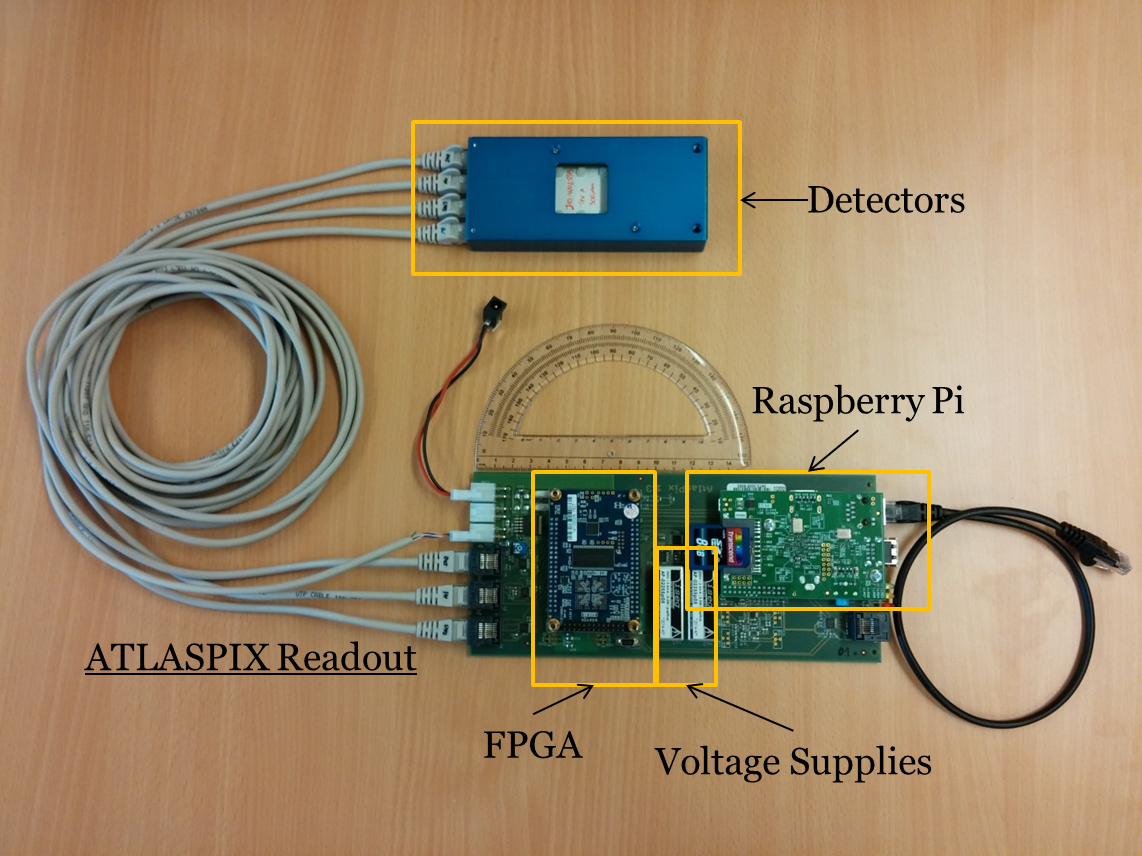
\includegraphics[height=7cm]{figures/imported/atlaspix}
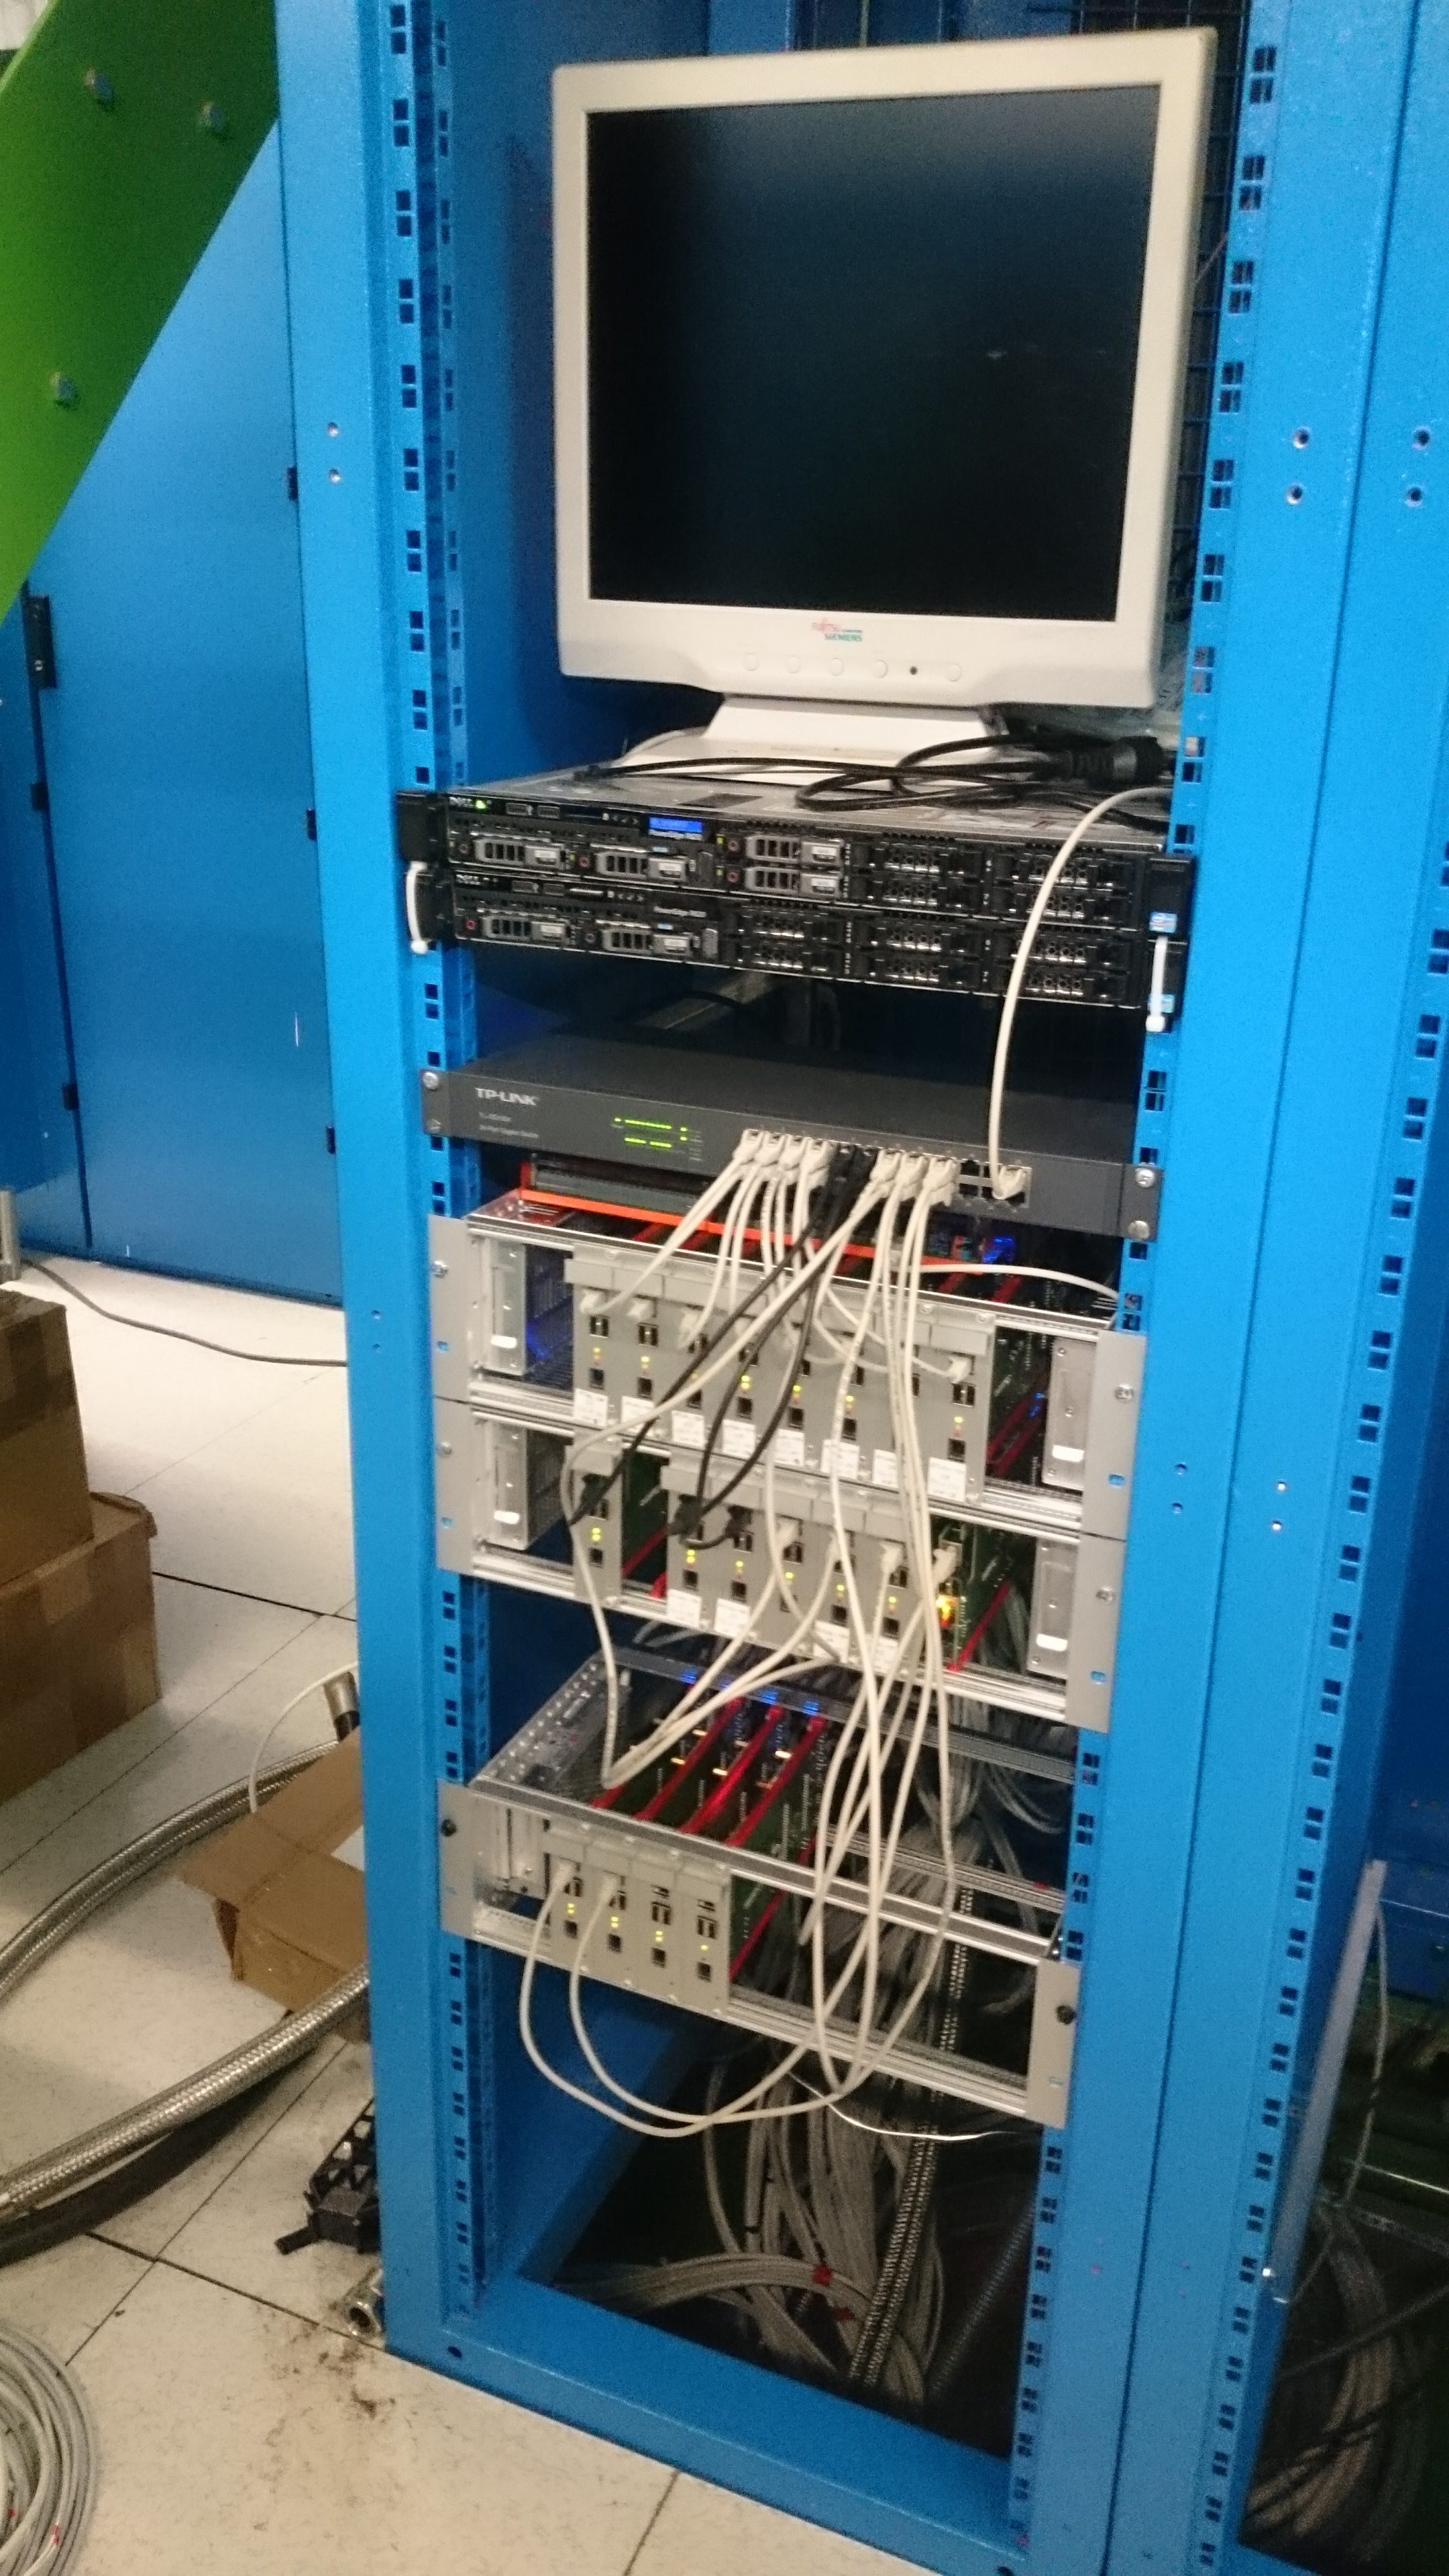
\includegraphics[height=7cm]{figures/imported/atlaspix-installed}
\caption{The ATLASPIX read-out interface installed at CERN.}
\label{fig:ATLASPIX}
\end{center}
\end{figure}


\subsection{Cluster Analysis}
%% CITACE: flood-fill
%% ZKRATKA: TOA, TOT
In ATLAS measurements, we strive to configure our detectors to capture frames containing multiple disconnected components corresponding with individual interacting particles. Naively speaking, we don't want our frames to be neither fully saturated, nor empty, but \textit{just right}. The task of achieving this level of balance is fairly straightforward, as it merely consists of fine-tuning the acquisition time parameter while monitoring levels of saturation in recently captured frames.

In well-balanced frames, we can then observe components of various shapes and sizes, depending on the experiments performed at the time of acquisition. These components, commonly known as \textit{clusters}, are discovered and evaluated in an automated process called \textit{the cluster analysis}. This procedure involves a connectivity-checking algorithm, such as \textit{flood-fill}, operating on pixel matrices to distinguish individual clusters. In later stages, clusters are processed, measured and classified in various categories with regards to their shape. In addition, if the frame has been captured in TOT mode and calibration data are available, the automated processing script can convert counter values to energy approximations.

%% OBR: saturovaný snímek - špatně (TPX01@1441600713.82345, 2015_09_07_TPX01.root, frame #16512)
%% OBR: snímek s clustery - dobře (TPX01@1435930709.35062, 2015_07_03_TPX01.root, frame #34979)

% CITACE: sparse matrix
The output of cluster analysis consists of two separate lists of clusters, one per every sensor layer. It follows from the definition of a cluster that any pixel contained in it has a non-zero counter value. Consequently, all pixels unreferenced by any cluster are assumed to be equal to zero. The utilized technique of data encoding is well-known as it offers efficient compression rate for sparse pixel matrices which we are expecting to encounter in our measured data. It is however worth noting at this point that in certain cases (represented most notably by saturated or nearly saturated frames), this approach produces voluminous data structures, which may take long time to enumerate, and in turn slow down other algorithms operating on them.

In a cluster list, pixels are stored as tuples of their Carthessian coordinates and their respective counter values. From this information, the pixel matrix can be reconstructed at any time. The original pixel matrix is therefore discarded at the end of the cluster analysis, in order to minimize occupied space. Please note that should there be any errors discovered in the future, data processed in this way could be still converted back into the form of pixel matrices by means of simple enumeration. Following that, a patched version of the cluster analysis process would analyze the pixel data once again, simply replacing any erroneous output with a correct one.

Let us now further inspect data generated by the process of cluster analysis. As we hinted at the beginning of this section, many other secondary values are calculated for every cluster during the automated processing, most notable of which are:

\begin{description}
	\item[Shape Classification]
	By measuring geometric properties of a cluster (such as radius or size), we are able to estimate whether the cluster resembles more a line segment or a circular blob. Similarly, we can also estimate if the cluster looks thin or thick. From that information, we can infer the type of interacting particle and direction of its movement relative to the plane of incidence. To formally define cluster categories, we will use terminology consistent with the ATLAS Medipix research (see Figure \ref{fig:cluster-types}).

    %% CITACE: Medipix cluster types

    \begin{figure}[t]
    \begin{center}

    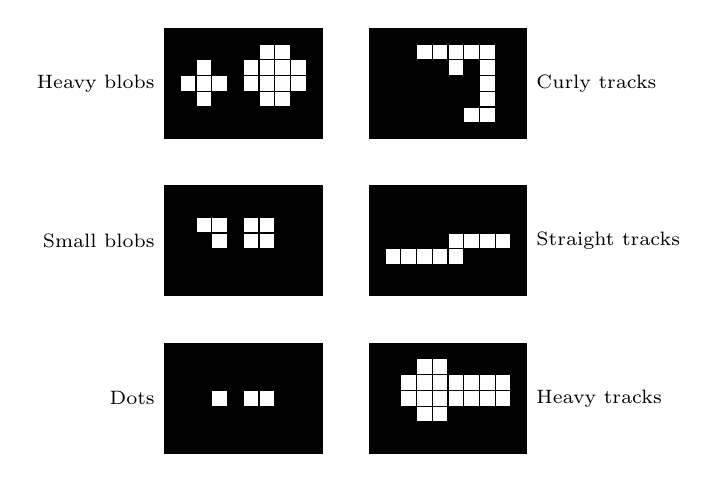
\begin{tikzpicture}
        % Dots
        \draw [fill=black] (0,0) rectangle (2,1.4);
        \draw [fill=white] (0.6,0.6) rectangle (0.8,0.8);
        \draw [fill=white] (1.0,0.6) rectangle (1.2,0.8);
        \draw [fill=white] (1.2,0.6) rectangle (1.4,0.8);
        \node[black,font=\scriptsize,anchor=east] at (0,0.7) {Dots};

        % Small blobs
        \draw [fill=black] (0,2) rectangle (2,3.4);
        \draw [fill=white] (0.6,2.6) rectangle (0.8,2.8);
        \draw [fill=white] (0.4,2.8) rectangle (0.6,3.0);
        \draw [fill=white] (0.6,2.8) rectangle (0.8,3.0);

        \draw [fill=white] (1.0,2.6) rectangle (1.2,2.8);
        \draw [fill=white] (1.2,2.6) rectangle (1.4,2.8);
        \draw [fill=white] (1.0,2.8) rectangle (1.2,3.0);
        \draw [fill=white] (1.2,2.8) rectangle (1.4,3.0);
        \node[black,font=\scriptsize,anchor=east] at (0,2.7) {Small blobs};

        % Heavy blobs
        \draw [fill=black] (0,4) rectangle (2,5.4);
        \draw [fill=white] (0.4,4.4) rectangle (0.6,4.6);
        \draw [fill=white] (0.2,4.6) rectangle (0.4,4.8);
        \draw [fill=white] (0.4,4.6) rectangle (0.6,4.8);
        \draw [fill=white] (0.6,4.6) rectangle (0.8,4.8);
        \draw [fill=white] (0.4,4.8) rectangle (0.6,5.0);

        \draw [fill=white] (1.0,4.6) rectangle (1.2,4.8);
        \draw [fill=white] (1.0,4.8) rectangle (1.2,5.0);
        \draw [fill=white] (1.2,4.4) rectangle (1.4,4.6);
        \draw [fill=white] (1.4,4.4) rectangle (1.6,4.6);
        \draw [fill=white] (1.2,4.6) rectangle (1.4,4.8);
        \draw [fill=white] (1.4,4.6) rectangle (1.6,4.8);
        \draw [fill=white] (1.2,4.8) rectangle (1.4,5.0);
        \draw [fill=white] (1.4,4.8) rectangle (1.6,5.0);
        \draw [fill=white] (1.2,5.0) rectangle (1.4,5.2);
        \draw [fill=white] (1.4,5.0) rectangle (1.6,5.2);
        \draw [fill=white] (1.6,4.6) rectangle (1.8,4.8);
        \draw [fill=white] (1.6,4.8) rectangle (1.8,5.0);
        \node[black,font=\scriptsize,anchor=east] at (0,4.7) {Heavy blobs};

        % Heavy tracks
        \draw [fill=black] (2.6,0) rectangle (4.6,1.4);
        \draw [fill=white] (3.0,0.6) rectangle (3.2,0.8);
        \draw [fill=white] (3.0,0.8) rectangle (3.2,1.0);
        \draw [fill=white] (3.2,0.4) rectangle (3.4,0.6);
        \draw [fill=white] (3.4,0.4) rectangle (3.6,0.6);
        \draw [fill=white] (3.2,0.6) rectangle (3.4,0.8);
        \draw [fill=white] (3.4,0.6) rectangle (3.6,0.8);
        \draw [fill=white] (3.2,0.8) rectangle (3.4,1.0);
        \draw [fill=white] (3.4,0.8) rectangle (3.6,1.0);
        \draw [fill=white] (3.2,1.0) rectangle (3.4,1.2);
        \draw [fill=white] (3.4,1.0) rectangle (3.6,1.2);
        \draw [fill=white] (3.6,0.6) rectangle (3.8,0.8);
        \draw [fill=white] (3.6,0.8) rectangle (3.8,1.0);
        \draw [fill=white] (3.8,0.6) rectangle (4.0,0.8);
        \draw [fill=white] (3.8,0.8) rectangle (4.0,1.0);
        \draw [fill=white] (4.0,0.6) rectangle (4.2,0.8);
        \draw [fill=white] (4.0,0.8) rectangle (4.2,1.0);
        \draw [fill=white] (4.2,0.6) rectangle (4.4,0.8);
        \draw [fill=white] (4.2,0.8) rectangle (4.4,1.0);
        \node[black,font=\scriptsize,anchor=west] at (4.6,0.7) {Heavy tracks};

        % Straight tracks
        \draw [fill=black] (2.6,2) rectangle (4.6,3.4);
        \draw [fill=white] (2.8,2.4) rectangle (3.0,2.6);
        \draw [fill=white] (3.0,2.4) rectangle (3.2,2.6);
        \draw [fill=white] (3.2,2.4) rectangle (3.4,2.6);
        \draw [fill=white] (3.4,2.4) rectangle (3.6,2.6);
        \draw [fill=white] (3.6,2.4) rectangle (3.8,2.6);
        \draw [fill=white] (3.6,2.6) rectangle (3.8,2.8);
        \draw [fill=white] (3.8,2.6) rectangle (4.0,2.8);
        \draw [fill=white] (4.0,2.6) rectangle (4.2,2.8);
        \draw [fill=white] (4.2,2.6) rectangle (4.4,2.8);
        \node[black,font=\scriptsize,anchor=west] at (4.6,2.7) {Straight tracks};

        % Curly tracks
        \draw [fill=black] (2.6,4) rectangle (4.6,5.4);
        \draw [fill=white] (3.2,5.0) rectangle (3.4,5.2);
        \draw [fill=white] (3.4,5.0) rectangle (3.6,5.2);
        \draw [fill=white] (3.6,5.0) rectangle (3.8,5.2);
        \draw [fill=white] (3.8,5.0) rectangle (4.0,5.2);
        \draw [fill=white] (4.0,5.0) rectangle (4.2,5.2);
        \draw [fill=white] (3.6,4.8) rectangle (3.8,5.0);
        \draw [fill=white] (4.0,4.8) rectangle (4.2,5.0);
        \draw [fill=white] (4.0,4.6) rectangle (4.2,4.8);
        \draw [fill=white] (4.0,4.4) rectangle (4.2,4.6);
        \draw [fill=white] (4.0,4.2) rectangle (4.2,4.4);
        \draw [fill=white] (3.8,4.2) rectangle (4.0,4.4);
        \node[black,font=\scriptsize,anchor=west] at (4.6,4.7) {Curly tracks};
    \end{tikzpicture}

    \caption{Different cluster types classified by their shapes.}
    \label{fig:cluster-types}
    \end{center}
    \end{figure}

	\item[Size, Volume]
	The size of a cluster is equal to the number of connected pixels which constitute it. The volume is a sum of counter values of those pixels.

	\item[Centroid, Volumetric Centroid]
	The centroid is defined as an unweighted average of pixel coordinates in the cluster. In analogous way, the volumetric centroid is the very same average weighted by corresponding counter values. 

	\item[Minimum and Maximum Cluster Height]
	These two figures refer to the lowest and the greatest counter values of pixels in the cluster.

	\item[Energy-based Properties \textit{(available only in TOT mode)}]
	If the energy approximations are available, many of the above-mentioned values can be also calculated with the energy substituted for counter values.
\end{description}

\section{Common Storage Formats}
\label{db:storage-formats}

\subsection{The Single-Frame and Multi-Frame Formats}
%  - Multi-frame formáty, jejich výhody a nevýhody.
The most straight-forward way of storing data acquired by Timepix detectors is to use plain text files. Such output, referred to as the single-frame or the multi-frame format, commonly stores data in three files per unit of acquisition.

\begin{description}
	\item[Data File]
	Data files contain captured data from individual pixels of the detector. The data is encoded as a simple list of tuples containing pixel positions and their respective counter values. All pixels which are not mentioned are assumed to be of zero value.

	\item[Description File]
	Description files contain configuration of the detector at the time of acquisition. While there is no exhaustive definition listing every serialized parameter, the description files allow to be easily extended by annotating values of parameters they store.

	To store a configuration parameter, three lines of text are required. The display name of the parameter (along with the unit or any other notes) is written on the first line. The second line describes the data type of the value and its range. The third line contains the actual value.

	\item[Index File]
	% TODO
	TODO
\end{description}

The text format has several advantages. Being encoded mostly in plain text files, data can be easily parsed without any software dependencies, and in case of possible corruption, files can be quickly checked in any text editor. Furthermore, since the format is directly produced by the Timepix read-out software, no additional data conversions are required.

With all these features in mind, this storage format is certainly not optimal on all fronts. Its nature brings about utterly wasteful storage strategies, particularly noticable in frequently repeated descriptive information. This inefficiency is even aggravated by not taking advantage of obvious benefits offered by binary serialization. Consequently, files stored in the multi-frame format tend to be quite large in size, often forcing users to split them into smaller time periods.

\subsection{The ROOT Format}
Another storage option is the ROOT Data Analysis Framework \cite{Brun199781}. Originally concieved at CERN in 1995, the framework provides a set of powerful tools with various applications in data mining, manipulation and visualization. Unlike other similar toolkits, ROOT comes with its own machine-independent binary file format (identified by the \texttt{.root} extension). This format is designed to store enormous amounts of data within various types of data structures efficiently, while maintaining good overall performance by employing low-level memory optimization techniques and multi-tier content caching.

%% ZKRATKA: API
%% ZKRATKA: ROOT?

Used by many physicists at CERN for several years now, ROOT seems like a good choice of a data archivation format as many researchers have already learned its caveats and know well how to operate it despite often lacking deeper background in Computer Science. For the purposes of programmatic access, ROOT also does well with documented APIs in Python, R and C++.

Should data be stored in ROOT, a basic relational database concept comes to mind. ROOT however offers even more abstract data structures with standard tables generalized in the form of \textit{trees} and their columns in the form of \textit{leaves}. One such tree would suffice for information about captured frames (such as acquisition time, operation mode, etc.) and other for a list of clusters for every frame. This schema (showcased in Figure \ref{fig:root-trees}) would efficiently abstract the entire storage structure, allowing for multiple frames to be stored in a single file, grouped for instance by a common time interval, similarly to the text file format.

\begin{figure}[t]
\begin{center}

\begin{tikzpicture}[
    every node/.style={
        draw=black,
        thick,
        anchor=west,
        inner sep=2pt,
        minimum size=1pt,
    },
    grow via three points={
        one child at (0.8,-0.7) and two children at (0.8,-0.7) and (0.8,-1.4)
    },
    edge from parent path={
        ($(\tikzparentnode\tikzparentanchor)+(.4cm,0pt)$) |- (\tikzchildnode\tikzchildanchor)
    },
    growth parent anchor=west,
    parent anchor=south west
  ]
  \node {\texttt{data.root}}
    child { node {\texttt{calibData}} 
    	child { node [draw=none] { Calibration constants } }
    	child { node [draw=none] { Detector position \& orientation } }
    }
    child [missing] {}
    child [missing] {}
    child { node {\texttt{dscData}} 
    	child { node [draw=none] { Frame 1 detector configuration } }
    	child { node [draw=none] { Frame 2 detector configuration } }
    	child { node [draw=none] { \ldots } }
    }
    child [missing] {}
    child [missing] {}
    child [missing] {}
    child { node {\texttt{clusterFile}}
    	child { node [draw=none] { Frame 1 cluster list } }
    	child { node [draw=none] { Frame 2 cluster list } }
    	child { node [draw=none] { \ldots } }
    };
\end{tikzpicture}

\caption{Structure of a ROOT file containing Timepix data.}
\label{fig:root-trees}
\end{center}
\end{figure}

In spite of being over 20 years in development, ROOT is not perfect. Using memory monitoring tools such as \cite{nethercote2007valgrind}, we have confirmed that the C++ implementation of the ROOT framework is riddled with various memory leaks, making it unsuitable for time-extensive operations. Some might also argue, that a full tree data structure might be overly-complicated and too generalized for a simple output described in previous sections. Lastly, ROOT framework has quite a complex object structure, making it hard to learn for first-time users.


\section{Proposed Data Structure}
Having defined the essence of information we wish to store and several data formats as means to do it, we are now ready to focus on the definition of our database. 

\subsection{Formal Requirements}
Requirements on such a data structure are as common as database requirements can get. It should be a reliable permanent storage element, accessible for reading from multiple workstations at a same time and robust enough to withstand minor hardware failures. With 15 detectors already installed at ATLAS, and possible option of installing another 5, the database should be designed to hold frames from up to 20 Timepix devices for the entire expected time period of their operation at LHC (that from June 2015 to LS3 in 2021).

% ZKRATKA: LHC
% CITACE: LHC schedule, LS2, LS3

As more and more frames arrive from the detector network, our database should allow to be periodically extended with new data, possibly processing and converting pixel matrices into cluster lists, as described in the previous sections. Since the database will be primary storage site for all research data, there should be multiple independent copies of it as backups and the database structure should be designed with logic to enable timely synchronization of these copies.

Apart from all the requirements already listed, we have the advantage of knowing how the majority of user queries will look like. With regards to this information, we may then optimize data storage and retrieval procedures to accelerate such queries. After discussing all use cases with the researchers who are going to operate the database, we have determined that most queries will filter data by time or by device. This is indeed a very natural method, provided that every device in the network is positioned and oriented in way allowing only for a certain type of particles to be observed. Researchers looking for signs of specific particles might often request data based on other experiments, which were conducted in a determinate time period and involved only a specific group of detectors in the network.


\subsection{Definition}
\label{db:definition}
With all requirements in mind, we will now formally define the database. Accounting for the ever-growing nature of our data, we will separate the database into two parts. The first part is to contain data which has already been processed by the cluster analysis, and is ready to be accessed by users. The second part will contain data which has arrived from CERN in its raw form but hasn't been processed yet. As one might note, this separation of data serves a fundamental purpose, that is to distinguish the intermediate products from the finished ones.

% ZKRATKA: UNIX
% ZKRATKA: HTTP
% ZKRATKA: SMB
% ZKRATKA: SSH
% ZKRATKA: AFP
% ZKRATKA: FTP
% ZKRATKA: EOS
% CITACE: UNIX file system

For simplicity, the database will be represented by a UNIX file system. This will enable many users, not necessarily only those using UNIX-based operating systems, to access it directly by means of widely-used and standardized protocols, such as FTP, SMB, SSH, AFP or HTTP\label{db:supported-protocols}. Utilization of these protocols contributes not only to the universality of our database, it also takes care of shared resource access and other data concurrency issues for us. Some of these features may prove to be useful later on when synchronizing various storage sites in order to back up or restore data. UNIX file systems also offer fundamental security features, allowing us to grant read-write privileges to a certain group of users, while limiting others to mere read-only access.

% CITACE: Označení TPX detektorů v ATLASu.

The file system will have two directories named \texttt{processed} and \texttt{downloading}, corresponding to the respective sections of the database. In these directories, data will be further grouped in subdirectories by the device of origin. To make navigation easier, device directory names will use numeric identifiers in compliance with already published literature. For instance, all data originating from the sensor no. 7 will be stored in a directory named \texttt{ATPX07}. In such directory, data will be stored in time-coded files (or directories, should multiple files be grouped under single time code) according to the naming pattern: \texttt{[yyyy]\_[mm]\_[dd]\_ATPX[id]} (where \texttt{[id]} is substituted for the device identifier and \texttt{[yyyy]}, \texttt{[mm]}, \texttt{[dd]} are substituted for year, month and day of the acquisition time respectively).

If it is not possible to group data by the day of acquisition for some reason, we define an alternative naming pattern with hourly granularity: \texttt{[yyyy]\_[mm]\_[dd]\_ATPX[id]\_[hh]} (where \texttt{[hh]} is substituted for the hour of acquisition and other entities are substituted in the same way as in the previous pattern). Note that in spite of grouping data files in separate subdirectories by the device of origin, we still include the device identifier in the naming pattern for reasons of redundancy.

The directory structure we have described so far satisfies all requirements we have stated in the previous section. What's more, it optimizes access to data generated from specific devices at specific times, so that the majority of user requests is satisfied in timely manner.

Let us now define the data files themselves. All data files will be stored at the lowest level of our directory structure and will have time-coded names according to our naming patterns. Should more files fall under the same time code (marginal scenario), they are to be grouped in a directory with a time-coded name. File structure in such a directory is undefined. We expect all files in the \texttt{processed} directory to be stored in the ROOT format, and all files in the \texttt{downloading} directory to be stored as multi-frames. All other files of different types will be tolerated as they may contain relevant information, but regarded as secondary. Further illustration of the file system can be found in Figure \ref{fig:db-structure}.

\begin{figure}[t]
\begin{center}

\begin{tikzpicture}[
    every node/.style={
        draw=black,
        thick,
        anchor=west,
        inner sep=2pt,
        minimum size=1pt,
    },
    grow via three points={
        one child at (0.8,-0.7) and two children at (0.8,-0.7) and (0.8,-1.4)
    },
    edge from parent path={
        ($(\tikzparentnode\tikzparentanchor)+(.4cm,0pt)$) |- (\tikzchildnode\tikzchildanchor)
    },
    growth parent anchor=west,
    parent anchor=south west
  ]
  \node {\textbf{Timepix Database/}}
    child { node {\texttt{downloading/}} }
    child { node {\texttt{processed/}}
    	child { node [draw=none] {\texttt{README.txt}} }
    	child { node {\texttt{ATPX01/}} }
    	child { node {\texttt{ATPX02/}}
    		child { node [draw=none] {\ldots}}
    		child { node [draw=none] {\texttt{2015\_08\_24\_ATPX02.root}} }
    		child { node [draw=none] {\texttt{2015\_08\_25\_ATPX02.root}} }
    		child { node {\texttt{2015\_08\_26\_ATPX02/}}
    			child { node [draw=none] {\texttt{morning.root}} }
    			child { node [draw=none] {\texttt{afternoon.root}} }
    			child { node [draw=none] {\texttt{evening.root}} }
    		}
    	}
    };
\end{tikzpicture}

\caption{Example of the database file system structure.}
\label{fig:db-structure}
\end{center}
\end{figure}

% ZKRATKA: zip
% ZKRATKA: tar

To preserve storage space, we will allow usage of data compression in our database. The supported compression formats are ZIP, GZIP and TAR, or any combination of them. As we expect the individual data files to grow quite large in size, we will utilize compression only at the lowest level of our directory structure, that is in the time-coded data files (or directories). Every archive can store at most one time-coded file (or directory), hence the archive can adopt the file's time-coded name, while remaining unique in the file listing. It is preferred, but not required, that all data files stored in a single directory are either all compressed or none of them is, as any deviation from this scheme might point to an incomplete or broken data transaction. Lastly, we forbid any recursively compressed structures (such as archive within other archive, etc.). The recommended alternative is to increase compression level in already existing archives instead of creating new ones. This rule also applies for all data formats which use compression inherently, such as ROOT.


\subsection{Expected Volume of Data}
With our definition in mind, we will now perform a simple extrapolation to obtain an upper bound on the size of our database.

Assuming that one hour of footage stored in the multi-frame format may take up to 4~gigabytes in size (depending on the frequency of acquisition), we have 96~gigabytes per sensor per day. Accounting for the longest possible time of operation, our database will store up to 2,437~days of footage simultaneously recorded by up to 20~detectors. That means that our database will have to hold about 4.7~petabytes worth of uncompressed information. If we use Collin's compression algorithm benchmark from \cite{GzipBenchmark} as baseline, it is possible to estimate that a common variant of GZIP algorithm will reduce the file size in average by 75.9\%. Applying this compression on our multi-frame data files, our database would have to hold \textit{only} about 1.1 petabyte of archives.

We will now perform analogous calculation for the ROOT file format. Since the file structure already utilizes its own proprietary compression algorithms, we expect the overall volume to decrease significantly in comparison with the raw uncompressed multi-frame data. From the data recorded by the ATLAS Timepix network in the fall of 2015, we observe that a single day of footage stored in the ROOT format may take up to 18~gigabytes in size. Using the same constants as before, we arrive at the conclusion that our database will have to hold about 877~terabytes of information. This result is in agreement with our expectations.

Please note that neither of these upper bounds is by any means, since we intentionally over-estimated the number of detectors in our network and the length of the operation period in our assumptions. In addition, it is likely that some of our detectors will be configured to capture data with frequencies lower than the maximum possible frequency as every device is configured separately to observe particles at different speeds. For all these reasons, our estimation only gives us vague information about the orders of magnitude of storage space required to operate our database and its subsequent backups. In spite of this limitation, the estimation suffices to design and rate other components of our system. 


\section{Index Database}
So far, we have established a set of rules for our file system, in order to quickly obtain data from a specific device captured at a specific time. These facilities are sufficient for navigating and accessing data in rudimentary manner, but are certainly not optimal. For instance, our rules do not define any conventions regarding retrieval of specific frames from files in the ROOT data format. Due to this limitation, users seeking individual frames will have to download bulks of data from longer time periods (their length can vary from an hour to a day in time and from hundreds of megabytes to several gigabytes in size), which may induce unnecessary processing overhead and memory shortages.

There is also no guarantee that time-coded nodes in our directory structure will be individual files. If such nodes happen to be directories, the file structure inside of such directories is undefined, and may require additional decisions on the user side. And what do we do when we want to retrieve frames based on different criteria than time and device of origin? At the moment, we have no option other than to directly enumerate frames stored in all files in our file system, which (considering their potential size) might not be a preferrable solution. To resolve all these issues, we will introduce one more element to our design---an index database.

This database will be contain information which can be recalculated at any instant from the primary data files, hence it will not need to be backed up. The information stored in our database will mostly include, as the name suggests, index of all files and frames on the record and addresses pointing to the them on our file system. In addition, the index database will also store some commonly requested aggregated values.



\subsection{Definition}
% ZKRATKA: SQL
The index database will be compliant to the SQL standard, so that users may design their own queries. For the reasons of simplicity, we will define only three basic entities in our database. The relationships between these entities are depicted in Figure \ref{db:index-uml}, whereas the meaning of their members is defined in this section.

% OBR: UML diagram databáze

\label{db:definition}
\begin{description}
	\item[Sensor]
	Sensor represents a single Timepix device, from which data can be acquired. For full definition of the SQL table, see Listing \ref{lst:sql-sensors}.

	\begin{description}
		\item[Sensor Identifier (\texttt{sid})]
		Identifier of the device, unique within the index database.

		\item[Name (\texttt{name})]
		Readable name of the sensor, consistent with the other literature.
		% CITACE: označení TPX detektorů v ATLASu

		\item[Calibration Constants (\texttt{calibration\_layer1}, \texttt{calibration\_layer2})]
		Constants used for luminosity calculation, available only for some devices.
	\end{description}

	\item[ROOT File]
	File represents a single file in the ROOT data format, containing data acquired from a single Timepix device in a determinate time period. For full definition of the SQL table, see Listing \ref{lst:sql-rootfiles}.

	\begin{description}
		\item[File Identifier (\texttt{fid})] 
		Identifier of the file, unique within the index database.

		\item[Device of Origin (\texttt{sid})]
		Identifier of the Timepix device, which acquired all data stored within this file.

		\item[File Path (\texttt{path})] 
		Absolute path to the file in the server's file system.

		\item[Date of Addition (\texttt{date\_added})]
		Date and time, when the file was added to the database.

		\item[Covered Time Interval (\texttt{start\_time}, \texttt{end\_time})]
		Minimum and maximum start time of the Timepix frames stored within this file.

		\item[Statistics (\texttt{count\_frames}, \texttt{count\_entries})]
		The total number of frames and clusters stored in within this file.

		\item[Validation Data (\texttt{checksum}, \texttt{date\_checked})]
		SHA1 checksum of the file and the latest date and time, when the file was validated against it to prevent data corruption.
	\end{description}

	\item[Frame]
	Frame represents a single event of data acquisition from a Timepix device. Every frame is stored in some file (and a file can contain multiple frames). For full definition of the SQL table, see Listing \ref{lst:sql-frames}.

	\begin{description}
		\item[Frame Identifier (\texttt{frid})] 
		Identifier of the frame, unique within the index database.

		\item[File Identifier (\texttt{fid})]
		Identifier of the file, in which the frame is stored.

		\item[Sensor Identifier (\texttt{sid})] 
		Identifier of the device, which captured this frame (must match \texttt{sid} of the file).

		\item[Start Time (\texttt{start\_time})] 
		Start time of the acquisition.

		\item[Acquisition Time (\texttt{acquisition\_time})] 
		Duration of the acquisition.

		\item[Data Addresses (\texttt{dsc\_entry}, \texttt{clstr\_first\_entry})]
		Index values pointing directly to entries within the ROOT file's internal structure, where the frame data is stored.

		\item[Statistics (\texttt{occupancy}, \texttt{clstr1\_count}, \dots, \texttt{clstr6\_count})]
		Total number of non-zero pixels in the frame, and numbers of clusters of different types in the frame.
	\end{description}
\end{description}


\subsection{Performance Optimization}
By the definition, it follows that our index database will help deterministically resolve all time-based queries, even in situations when frames are stored in an undefined directory structure. Apart from this optimization, the database will also provide file validation primitives to ensure that any corrupted files are discovered as soon as possible. But there is one more significant performance optimization we have so far neglected to mention.

When retrieving frames by the time and device of origin, we can use the predefined naming patterns to obtain a path in the file system. In case the path points to a directory, we can consult the index database to quickly scan for a file containing the information we need. Still, we are left with an unoptimized task since in order to retrieve the specific frame (or frames) we are looking for, we will have to scan the entire file, which may be several gigabytes in size.

This issue may be in part resolved by sorting all frames in our data files consistently by their start time, allowing us to use a binary search algorithm instead of regular one, thus reducing the complexity of the operation from linear to logarithmic. But we can still do better. Since we already perform lookups in the index database, we can us them to retrieve data addresses, which will point us to specific locations in the file. This way, no search will be needed at all.

Recall that ROOT files contain two trees of interest, the \texttt{dscData} tree with information about detector configuration, and the \texttt{clusterFile} tree, which contains concatenated lists of clusters from every frame. There is only one entry per frame in the \texttt{dscData} tree, whereas the \texttt{clusterFile} tree may contain anywhere from zero to hundreds of thousands of entries in a single frame. Entries belonging to the same frame can be identified by having equal value of the \texttt{Start\_time} leaf. If we agree to sort all entries in both trees by this leaf value, the \texttt{clusterFile} entries will consequently form continuous bulks of data corresponding to individual frames. This means that once we discover the bulk belonging to the frame we want, we only need to read entries as long as the start time remains the same (or we reach the last entry). For every frame, we can then store the index of the corresponding \texttt{dscData} entry and the index of the first \texttt{clusterFile} entry in the bulk to achieve constant-time search operation, as illustrated in Figure \ref{fig:db-index-optimization}. This significant benefit comes at the price of increased complexity of the insert operation due to additional sorting of entries in our files, and slightly increased space occupied by the index database because of stored entry indices.

\begin{figure}[t]
\begin{center}
\begin{tikzpicture}[
    >=stealth,
    node distance=3cm,
    database/.style={
      cylinder,
      shape border rotate=90,
      aspect=0.25,
      minimum width=2.5cm,
      minimum height=1.5cm,
      draw
    },
    mymat/.style={
      matrix of math nodes,
      text height=2.5ex,
      text depth=0.75ex,
      text width=3.25ex,
      align=center,
      column sep=-\pgflinewidth,
      row sep=-\pgflinewidth
    }]
    % The DB.
    \node[database] (db1) at (0,0) {Index DB};

    % The array.
	\matrix[mymat,anchor=west,row 2/.style={nodes=draw},below of=db1,row 1 column 4/.style={nodes={draw,fill=gray!30}},row 2 column 4/.style={nodes={draw,fill=gray!30}},row 2 column 5/.style={nodes={draw,fill=gray!30}},row 2 column 6/.style={nodes={draw,fill=gray!30}},row 2 column 7/.style={nodes={draw,fill=gray!30}}] (rootfile)
	{
		0  &  1 &  2 &  \textbf{3} &  4 &  5 &  6 &  7 &  8 &  9 & 10 & \dots \\
		29 & 29 & 31 & 32          & 32 & 32 & 32 & 33 & 37 & 40 & 40 & \dots \\
	};

	% Arrow connecting DB and the array.
	\draw[-{Stealth[scale=2.0]},black!100] (db1) -| node[black,above,font=\scriptsize,anchor=east]{\texttt{clstr\_first\_entry=3}} (rootfile-1-4.north);

	% Array labels on the left.
	\node[black,font=\scriptsize,left of=rootfile-1-1,node distance=5mm,anchor=east]{Entry Index};
	\node[black,font=\scriptsize,left of=rootfile-2-1,node distance=5mm,anchor=east]{Start Time [s]};

	% Label in the bottom.
	\node[black,font=\scriptsize,below of=rootfile,node distance=1cm,anchor=north]{\texttt{clusterFile} Tree};
\end{tikzpicture}

\caption{Illustration of the optimization mechanism provided by the index database.}
\label{fig:db-index-optimization}
\end{center}
\end{figure}


\subsection{Data Aggregation and Metaindexing}
In some cases, users of our database may want to calculate aggregated statistics. Since these types of requests are hard to anticipate and do not constitute a significant portion of all user queries, it is not worth our effort to create separate data structures in order to accelerate their processing. We can, however, make use of data structures we already have in place. For instance, our index database makes a great candidate in particular since it already contains data associated with individual files and frames, and is easily accessible and queriable using SQL. We will therefore include several statistical values, such as count of clusters differentiated by individual cluster types and frame occupancy encoded as number of non-zero pixels.

Users can utilize filtering and aggregation features of SQL to quickly find files and frames in the index database, and if required, analyze their contents more thoroughly.

Lastly, SQL implementations include an analogy to the index mechanism we used to accelerate our access to individual frames within data files. Using their own tree indices built from various columns of data tables, servers can speed up certain queries containing predicates or orderings based on such columns. We can utilize this mechanism to make our data access procedure even faster, in a sense indexing the index database. To see how exactly we make use of this technique, examine Listings \ref{lst:sql-sensors}, \ref{lst:sql-rootfiles} and \ref{lst:sql-frames}.


